\begin{frame}{Motivation}
  \begin{itemize}
    \item Traditional NLP models are \textbf{unimodal}: text in, text out; they can neither see nor hear the world their language describes.
    \item Human communication is grounded in perception: much of what language refers to arrives through vision, sound, and the other senses.
    \item \textbf{Vision-language models} align images with text at web scale, and today's assistants are \textbf{multimodal LLMs} built on top of that alignment.
    \item This lecture builds from contrastive alignment (CLIP and its successors) to the projector-and-instruction recipe behind multimodal assistants, and on to the natively multimodal and omni models of 2025--2026.
  \end{itemize}
\end{frame}

\begin{frame}{What is multimodality?}
  \begin{columns}[T,onlytextwidth]
    \column{0.62\textwidth}
      \vspace{-1ex}
      {\Large\bfseries multimodal \textit{adjective}}

      \vspace{0.3em}
      \textit{[ muhl-tee-moh-duhl ]}
      
      \vspace{0.4em}
      : having or involving several modes, modalities, or maxima

      \vspace{0.18em}
      \textit{multimodal distributions}

      \textit{multimodal therapy}
      
      \vspace{1.2em}
      {\small
      In our case, focusing on NLP: text + one or more other \textit{modality} (images, speech, audio, olfaction, others). We'll mostly focus on images as the other modality.
      }

    \column{0.34\textwidth}
      \begin{figure}
        \centering
        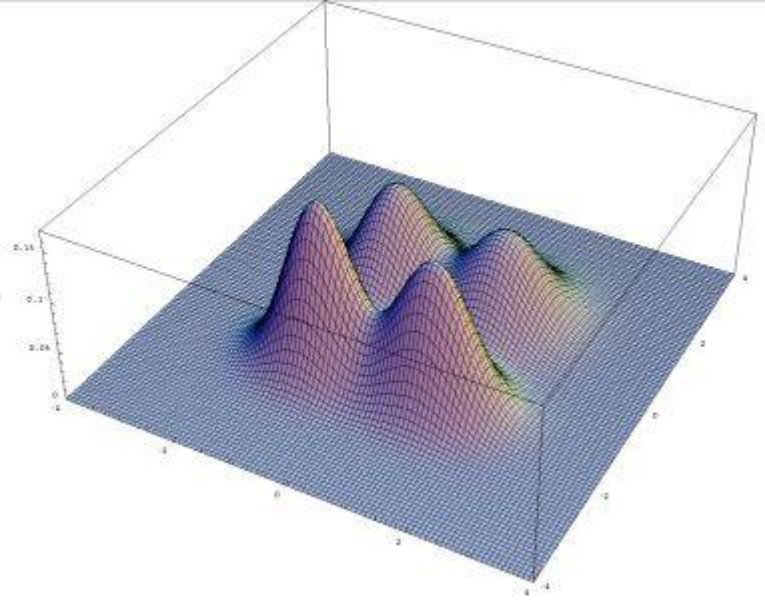
\includegraphics[width=0.75\linewidth, height=0.55\textheight, keepaspectratio]{images/multimodal-nlp/multimodal_gaussian_surface_plot.png}
        \caption*{\scriptsize A multimodal distribution: several maxima. Definition: Merriam-Webster, ``multimodal''.}
      \end{figure}
  \end{columns}
\end{frame}

\begin{frame}{Multimodal brains}
  \begin{itemize}
    \item \textbf{McGurk effect} (McGurk \& MacDonald, 1976)
      \begin{itemize}
        \item Classic demonstration of interaction between modalities (audio + vision) in perception
        \item Speech sound is misheard depending on visual (lip movement) cues
      \end{itemize}
    \item \href{https://www.youtube.com/watch?v=2k8fHR9jKVM}{Watch this demonstration on YouTube}
  \end{itemize}
  \vspace{0.5em}
  \begin{figure}
    \centering
    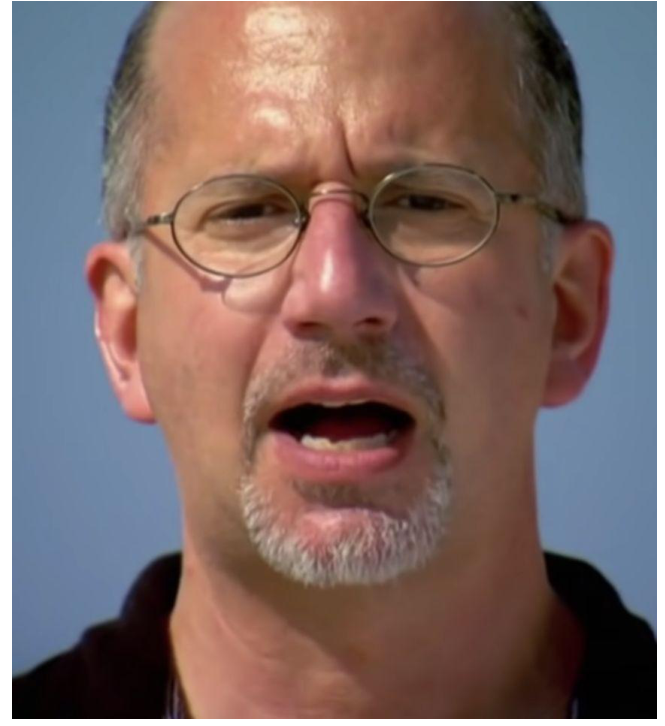
\includegraphics[width=0.42\textwidth, height=0.46\textheight, keepaspectratio]{images/multimodal-nlp/multimodal_speaking_person_video_frame.png}
    \caption*{\scriptsize Source: frame from ``McGurk effect: Auditory Illusion'', BBC \emph{Horizon}.}
  \end{figure}
\end{frame}

\begin{frame}{Why Ground Language in Perception?}
  \begin{itemize}
    \item \textbf{The symbol grounding problem} (Harnad, 1990): ``How can the semantic interpretation of a
      formal symbol system be made \emph{intrinsic} to the system, rather than just parasitic on the
      meanings in our heads?'' Harnad likens learning from symbols alone to learning Chinese from a
      Chinese-Chinese dictionary.
    \item \textbf{The octopus test} (Bender \& Koller, ACL 2020): a deep-sea octopus O taps the telegraph
      cable between two islanders and learns to impersonate one of them purely from the statistics of
      their messages. The act holds until real-world help is needed: ``having only form available as
      training data, O did not learn meaning.''
    \item Their conclusion: a system trained only on \emph{form} has a priori no way to learn
      \emph{meaning}; to learn language, it ``must solve what Harnad (1990) calls the symbol grounding
      problem.''
    \item Multimodal NLP is the constructive response: tie language to what the system can see and hear.
  \end{itemize}
  \vspace{0.3em}
  {\scriptsize Harnad, \emph{Physica D} 42:335--346, 1990;
  Bender \& Koller, ACL 2020, \href{https://aclanthology.org/2020.acl-main.463/}{aclanthology.org/2020.acl-main.463}.}
\end{frame}

\begin{frame}{A Decade of Multimodal NLP}
  \small
  \begin{tabular}{@{}p{1.2cm}p{12.1cm}@{}}
    \textbf{2015} & Captioning and VQA become benchmark tasks: Show and Tell (CVPR 2015), VQA (ICCV 2015) \\[0.25em]
    \textbf{2019} & BERT-style vision-language pretraining: ViLBERT (NeurIPS 2019), LXMERT (EMNLP 2019) \\[0.25em]
    \textbf{2021} & Contrastive alignment at web scale: CLIP (ICML 2021) \\[0.25em]
    \textbf{2022} & Few-shot multimodal in-context learning: Flamingo (NeurIPS 2022) \\[0.25em]
    \textbf{2023} & Visual instruction tuning (LLaVA); frontier chatbots gain vision (GPT-4V system card, Sep 2023) \\[0.25em]
    \textbf{2024} & Natively multimodal frontier models: GPT-4o, one network end-to-end across text, vision and audio \\[0.25em]
    \textbf{2025} & Images enter the chain of thought (o3); open omni models; native image generation \\[0.25em]
    \textbf{2026} & Native multimodality becomes the default in frontier and open releases alike \\
  \end{tabular}
  \vspace{0.6em}

  {\scriptsize Every milestone above is cited in the references.}
\end{frame}
